\documentclass[a4paper,12pt]{article}
\usepackage[utf8]{inputenc}
\usepackage[francais]{babel}
\usepackage[T1]{fontenc}
\usepackage{graphicx}
\usepackage{listingsutf8}
\usepackage[colorlinks,urlcolor=blue]{hyperref} %hyperlinks
% \usepackage[nottoc,notlot,notlof]{tocbibind} %To bind the table of contents to the bibligoraphy
% \usepackage[page,toc,titletoc,title]{appendix} %To add appendices to the document
\usepackage{../../packages/tikz-uml} %UML elements

\title{
  HMIN122M Rendu \\
  \large TP2
}
\author{Bachar Rima \and Joseph Saba \and Tasnim Muhammad}
\date{\today}

\lstset{
  language=SQL,
  basicstyle=\ttfamily\small,
  keywordstyle=\color{blue!60},
  commentstyle=\color{red!80}\upshape,
  stringstyle=\color{purple},
  showstringspaces=false,
  rulecolor=\color{black!30},
  numberstyle=\footnotesize,
  numbers=left,
  breaklines=true,
  breakatwhitespace=true,
  tabsize=3,
  frame=single,
  framextopmargin=2pt,
  framexbottommargin=2pt,
  backgroundcolor=\color{gray!10},
  captionpos=b,
  inputencoding=utf8,
  extendedchars=true,
  literate={á}{{\'a}}1 {é}{{\'e}}1 {í}{{\'i}}1 {ó}{{\'o}}1 {ú}{{\'u}}1 {Á}{{\'A}}1 {É}{{\'E}}1 {Í}{{\'I}}1 {Ó}{{\'O}}1 {Ú}{{\'U}}1 {à}{{\`a}}1 {è}{{\`e}}1 {ì}{{\`i}}1 {ò}{{\`o}}1 {ù}{{\`u}}1 {À}{{\`A}}1 {È}{{\'E}}1 {Ì}{{\`I}}1 {Ò}{{\`O}}1 {Ù}{{\`U}}1 {ä}{{\"a}}1 {ë}{{\"e}}1 {ï}{{\"i}}1 {ö}{{\"o}}1 {ü}{{\"u}}1 {Ä}{{\"A}}1 {Ë}{{\"E}}1 {Ï}{{\"I}}1 {Ö}{{\"O}}1 {Ü}{{\"U}}1 {â}{{\^a}}1 {ê}{{\^e}}1 {î}{{\^i}}1 {ô}{{\^o}}1 {û}{{\^u}}1 {Â}{{\^A}}1 {Ê}{{\^E}}1 {Î}{{\^I}}1 {Ô}{{\^O}}1 {Û}{{\^U}}1 {œ}{{\oe}}1 {Œ}{{\OE}}1 {æ}{{\ae}}1 {Æ}{{\AE}}1 {ß}{{\ss}}1 {ű}{{\H{u}}}1 {Ű}{{\H{U}}}1 {ő}{{\H{o}}}1 {Ő}{{\H{O}}}1 {ç}{{\c c}}1 {Ç}{{\c C}}1 {ø}{{\o}}1 {å}{{\r a}}1 {Å}{{\r A}}1 {€}{{\euro}}1 {£}{{\pounds}}1 {«}{{\guillemotleft}}1 {»}{{\guillemotright}}1 {ñ}{{\~n}}1 {Ñ}{{\~N}}1 {¿}{{?`}}1
}

\begin{document}
\pagestyle{plain}

\maketitle

{
  \hypersetup{linkcolor=black}
  \tableofcontents
}

\section{Sélection}
\subsection{Question 1}
\begin{description}
  \item [@script\_table.sql :] création des tables de la base de données.
  \item [@script\_remplissage.sql :] remplissage des tables crées.
  \item [set autotrace on :] permettre de faire des statistiques sur les requêtes exécutées.
  \item [set linesize 200 :] étendre la taille des tables affichées pour une meilleure visibilité.
\end{description}

\subsection{Question 2}
\begin{lstlisting}[caption={plan d'exécution choisi par l'optimiseur pour la requête permettant d'afficher le nom des villes dont le numéro insee est 34172}]
  explain plan for select nom from ville where insee='34172';
  select plan_table_output from table(dbms_xplan.display());
\end{lstlisting}

\begin{figure}[!ht]
  \centering
  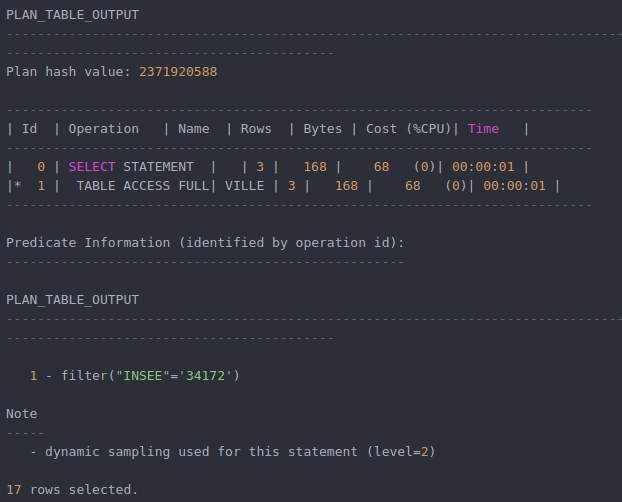
\includegraphics[scale=0.6]{images/q2_1.png}
  \caption{Plan d'exécution}
\end{figure}

\begin{figure}[!ht]
  \centering
  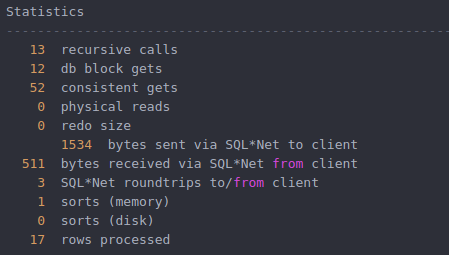
\includegraphics[scale=0.6]{images/q2_2.png}
  \caption{Statistiques}
\end{figure}

\newpage

\subsection{Question 3}
\begin{lstlisting}[caption={ajout d'une clé primaire sur la table ville en utilisant l'attribut insee}]
  alter table ville add constraint PK_VILLE PRIMARY KEY(insee);
\end{lstlisting}

\subsection{Question 4}
Avant l'ajout d'une clé primaire à la table \texttt{Ville}, l'algorithme choisi par l'optimiseur pour optimiser la requête est \textit{Table Access Full}. Ce dernier est généralement gourmand en termes de consommation de ressources, vu qu'il doit balayer la table entièrement, ligne par ligne, et attribut par attribut.

Après l'ajout d'une clé primaire à la table \texttt{Ville}, notamment sur l'attribut \textbf{insee}, l'algorithme choisi par l'optimiseur est ainsi \textit{Index Unique Scan}. Ce dernier permet de parcourir la table selon l'indexe placé sur la clé primaire et est ainsi moins gourmand en termes de consommation de ressources.

\section{Jointure}
\subsection{Question 5}
\begin{lstlisting}[caption={plan d'exécution choisi par l'optimiseur pour la requête permettant d'afficher le nom du département pour la ville dont le numéro insee est 34172}]
  explain plan for select departement.nom from departement, ville where insee='34172' and departement.id = ville.dep;
  select plan_table_output from table(dbms_xplan.display());
\end{lstlisting}

\begin{figure}[!ht]
  \centering
  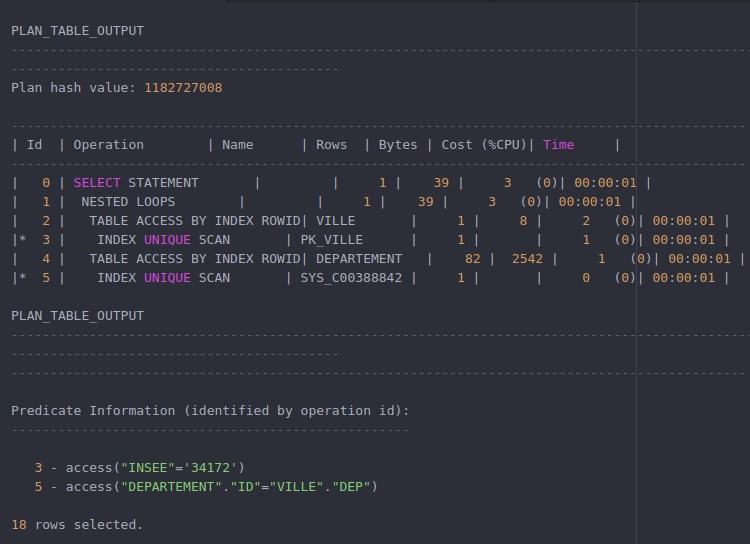
\includegraphics[scale=0.6]{images/q5_1.png}
  \caption{Plan d'exécution}
\end{figure}

\begin{figure}[!ht]
  \centering
  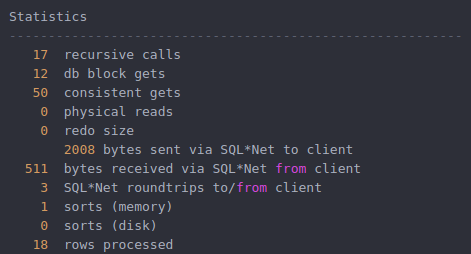
\includegraphics[scale=0.6]{images/q5_2.png}
  \caption{Statistiques}
\end{figure}

\subsection{Question 6}
Dans la requête précédente, nous avons utlisé les algorithmes \textit{Index Unique Scan} puis \textit{Nested Loops} lors de l'opération de jointure sur les tables \texttt{Ville} et \texttt{Departement}, vu que la jointure se fait sur les attributs clés primaires, respectivement \textbf{insee} et \textbf{id} de ces deux tables, après avoir sélectionné les tuples vérifiant une condition de sélection (en particulier, la ville ayant le code \textbf{insee} $34172$).

D'autre part, la requête courante ne spécifie aucune condition de sélection précédant la jointure sur les deux tables et utilise ainsi, respectivement, les algorithmes \textit{Table Access Full} pour balayer les tables et \textit{Hash Join} pour faire la jointure.

\begin{lstlisting}[caption={plan d'exécution choisi par l'optimiseur pour la requête permettant d'afficher le nom du département pour toutes les villes}]
  explain plan for select departement.nom from departement, ville where departement.id = ville.dep;
  select plan_table_output from table(dbms_xplan.display());
\end{lstlisting}

\begin{figure}[!ht]
  \centering
  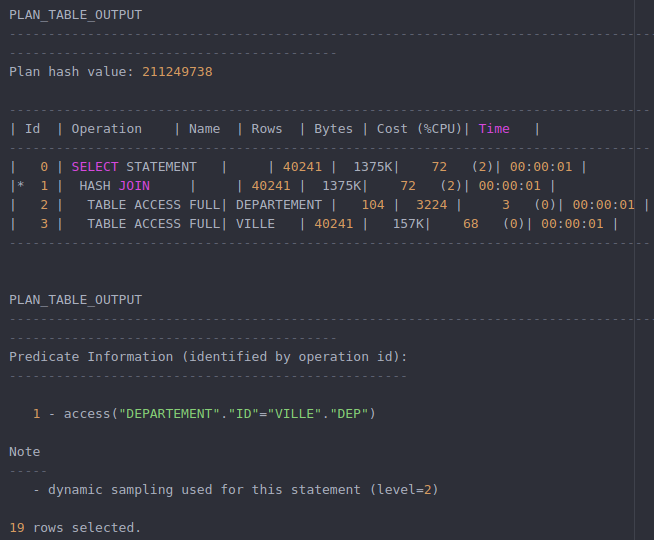
\includegraphics[scale=0.6]{images/q6_1.png}
  \caption{Plan d'exécution}
\end{figure}

\begin{figure}[!ht]
  \centering
  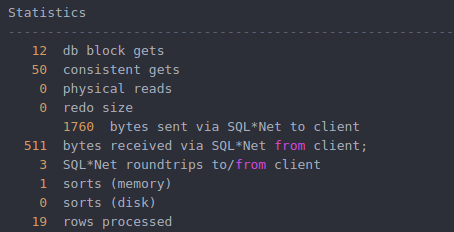
\includegraphics[scale=0.6]{images/q6_2.png}
  \caption{Statistiques}
\end{figure}

\subsection{Question 7}
\begin{lstlisting}[caption={plan d'exécution choisi par l'optimiseur pour la requête permettant d'afficher le nom des villes et du département dont le numéro est 91 (id)}]
  explain plan for select ville.nom, departement.nom from ville, departement where departement.id='91' and ville.dep=departement.id;
  select plan_table_output from table(dbms_xplan.display());
\end{lstlisting}

\begin{figure}[!ht]
  \centering
  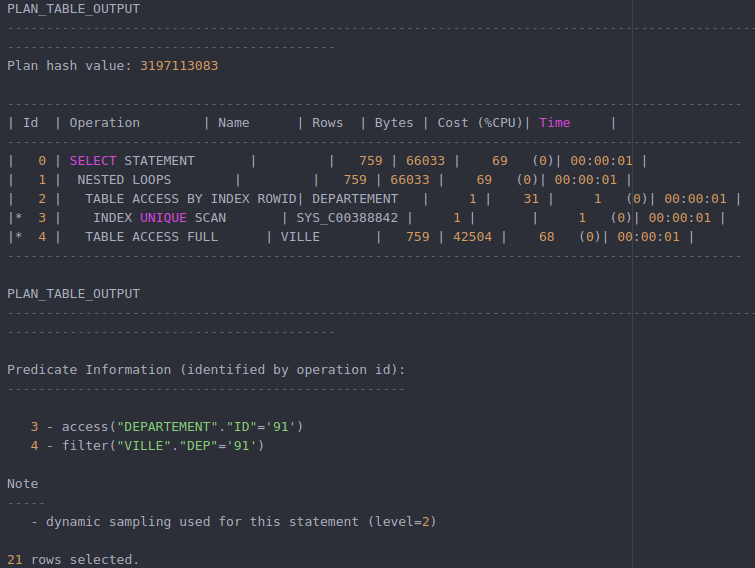
\includegraphics[scale=0.6]{images/q7_1.png}
  \caption{Plan d'exécution}
\end{figure}

\begin{figure}[!ht]
  \centering
  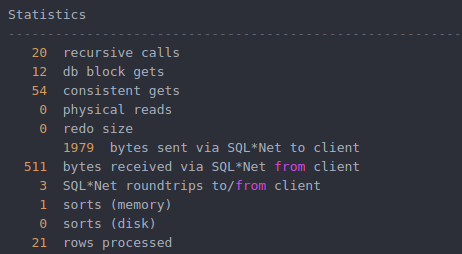
\includegraphics[scale=0.6]{images/q7_2.png}
  \caption{Statistiques}
\end{figure}

\section{Modification du comportement de l'optimiseur}
\subsection{Question 8}

\section{Utilisation d'index}
\subsection{Question 9}

\subsection{Question 10}

\subsection{Question 12}

\subsection{Question 13}

\section{Les statistiques des tables}
\subsection{Question 14}

\end{document}
